\documentclass[14pt]{matmex-diploma-custom}

\usepackage{amsthm}
\usepackage{amssymb}
\usepackage{amsmath}

\begin{document}
\filltitle{ru}{
    chair              = {Кафедра информационно-аналитических систем},
    title              = {Тут будет тема},
    type               = {coursework},
    author             = {Трофимов Артем Владимирович, Маршалкин Никита Евгеньевич},
    supervisorPosition = {к.\,ф.-м.\,н., доцент},
    supervisor         = {Кураленок И.\,Е.},
    faculty            = {Математико-механический факультет}
}
\filltitle{en}{
    chair              = {Sub-Department of Analytical Information Systems},
    title              = {Placeholder},
    type               = {coursework},
    author             = {Artem Trofimov, Marshalkin Nikita},
    supervisorPosition = {assistant professor},
    supervisor         = {Igor Kuralenok},
    faculty            = {Mathematics And Mechanics Faculty}
}
\maketitle

\tableofcontents

\section{Модель и архитектура}

Главная сущность системы - это поток данных протекающий через граф, узлами которого являются операции, последовательные применяемые к данным, а ребра задают порядок выполнения.

Нагрузка распределяется по хешу от данных, то есть на каждом вычислительном модуле выполняется весь граф, а пересылка между ними происходит, если данные поменяли хеш. Благодаря этому горизонтальная масштабируемость достигается без внесения изменений в бизнес-логику.

Источником данных является фронт, процесс работающий на клиенте: на веб-фронте, на каком-либо сенсоре. Поскольку между порождением данных и попаданием в систему нет посредников, появляются полезные свойства: отсутствует задержка, которую не избежать при использовании брокеров сообщений (Apache Kafka), каждый входной элемент можем пометить “своим” временем, что вносит детерминизм, при повторной обработке гарантируется такой-же результат. Так же наличие единого времени позволяет отойти от концепции micro-batching, “выпускать” обработанные элементы из системы до завершения окна (транзакции, batch’а).

Состояние системы и координационная информация хранится в  Apache Zookeeper, тем самым делегируя проблемы распределенного консенсуса.

\subsection{Время}

В нашей системе мы различаем два времени: глобальное и локальное.

\textbf{Глобальное время} - время входа элемента в систему в наносекундах с начала эпохи. Важно, что время - строго монотонно в рамках одного фронта и два разных события имеют разное время независимо от фронта. Первое условие достигается использованием  монотонных часов (CLOCK\_MONOTONIC). Чтобы обеспечить различие времени на разных фронтах во время вносится номер фронта.

\[GlobalTime := (frontTs, frontId)\]

Глобальное время сравнивается лексикографически: время, потом номер фронта.

Гарантии на синхронизацию времени не требуется для корректной работы, в отличии, например от Spanner [ссылка], но от этой разницы зависит нижняя граница задержки между событием и реакцией на него (появления данных на источнике и полной обработки).

\textbf{Локальное время} - логическое время каждой операции. В отличии от глобального, от него требуется лишь строгая монотонность во времени, то есть достаточно счетчика, увеличивающегося при обработке событий.

Некоторые операции могут порождать несколько элементов из одного, например  выпрямляющее отображение. Чтобы различать результаты к локальному времени добавим номер ребенка. Для отображений 1 в 1 номер ребенка будет равен нулю.

\[LocalEvent := (localTime, childId)\]

Аналогично глобальному времени локальное событие будем сравнивать лексикографически: вначале локальное время, потом номер ребенка.

Таким образом в каждый момент времени c каждым элементом протекающем по графу ассоциирована мета-информация: глобальное время и массив локальных времен операций, через который прошел элемент к данному времени.

\[Trace := [LocalEvent]\]
\[Meta := (GlobalTime, Trace)\]
\[DataItem := (payload, Meta)\]

В дальнейшем DataItem будем называть элементом. Будет подразумеваться, что у него есть некоторое глобальное время и след, может быть пустой, если он только что был порожден на фронте.

Мета-информацию будем сравнивать тоже лексикографически: глобальное время, потом след. В дальнейшем будет введено еще несколько порядков на мета-информации. Данный назовем естественным порядком.

\subsection{Операции}

Для построения логического графа используется следующий ограниченный набор операций:

\begin{itemize}
  \item отображение без состояния (map)
  \item выпрямляющее отображение (flatMap)
  \item группировка с окном по хешу (group)
  \item репликация (broadcast)
  \item слияние (merge).
\end{itemize}

\textbf{Отображение без состояния} применяет заданную функцию к входному элементу. Выходной элемент имеет глобальное время входного. А к следу прибавляется локальное время узла. Как понятно из названия, эта операция не имеет внутреннего состояния. Обработка двух элементов не зависит ни от порядка ни от локальности.

\textbf{Выпрямляющее отображение} сопоставляет каждому входному элементу множество выходных. Каждый элемент выходного множества впоследствии рассматривается как независимый. Все выходные элементы имеют глобальное время входного, к следу добавляется одинаковое локальное время но разный номер ребенка.

\textbf{Группировка с окном по хешу} последовательности входных элементов сопоставляет последовательность кортежей, размером с окно. Группировка в разных хешах выполняется независимо.

Например, если на вход подается последовательность натуральных чисел: \(1, 2, 3...\) , хешем является четность числа и окно - 3, то на выходе будет следующий набор кортежей:

\[(1), (2), (1|3), (2|4), (1|3|5), (2|4|6), (3|5|7)...\]

В отличии от партицирования по хешу, в данном случае хеш является частью логики. При этом хеш самой операции, который задает партицирование имеет смысл делать равным логическому хешу группинга.

Группировка - единственная операция в нашей системе обладающая состоянием - текущая история по хешу. Соответветственно результат операции зависит от порядка входных элементов, но результаты разных хешей независимы друг от друга. Гарантируется, что в рамках хеша результат будет такой же, каким был бы, если элементы на вход подаются в соответствии с глобальным временем. Про то, как это было получено будет рассказано в следующей главе.

Важным свойством такой семантики является то, что результат группировки однозначно определяется последним элементом в кортеже. Следовательно группировка это биективное отображение. Будем говорить, что этот кортеж защищается своим последним элементом.

Глобальным временем выходного элемента является глобальное время последнего элемента в кортеже. Следом - след последнего плюс локальное время группировки.

\textbf{Слияние} - операция с конечным числом входов и одним выходом. Каждый элемент с каждого входа подается на выход. Никаких гарантий на порядок не дается. К следу элемента добавляется локальное время операции.

\textbf{Репликация} обладает одним входном и множеством выходов.  Каждый элемент с входа подается, реплицируется на каждый выход. Аналогично выпрямлению все выходные элементы имеют глобальное время входного, к следу добавляется одинаковое локальное время но разный номер ребенка.

\begin{figure}
  \centering
	
\includegraphics[width=0.7\textwidth]{pics/ops.png}
	\caption{Операции}
\end{figure}

\subsection{Поддержание семантики группировки}

При исполнении графа на кластере, операции разнесены по разным физическим хостам, более того на одной машине операции разнесены по разным потокам. В графе возможны репликации, слияния, циклы. В этих условиях невозможно поддерживать порядок элементов, которые подаются на вход операций.

К счастью единственной операцией для которой принципиален порядок входных данных - группировка.

Для поддержания семантики каждая операция группировки будет хранить всю историю элементов, которые были поданы на вход. Назовем эту историю буфером. Поскольку группировка по различным хешам независима, такой буфер будет различным для каждого хеша. Элементы в буфере будут храниться в порядке порождения, то есть отсортированы по глобальному времени. В главе “Минимальное время” будет показана оптимизация, позволяющая чистить буфер.

Как только приходит новый элемент он вставляется в правильную позицию в буфер. Если он самый новый в буфере, пришел в правильном порядке, то собирается обычный кортеж размером с окно и подается на выход. Если же он не самый старый, то инициируется перепроигрывание. Начинают заново порождаться кортежи, которые содержат новоприбывший элемент.

Таким образом группировка рано или поздно породит корректные кортежи. Проблемой является то, что в потоке так же будут находиться и некорректные. В этой главе мы введем необходимые определения и покажем, как определяется и удаляются некорректные элементы. Для этого достаточно будет сравнивать мета-информацию элементов.

\subsubsection{Отношение зависимости}

Введем на множестве элементов отношение зависимости.

Элемент \(d_1\) зависит от \(d_0\) тогда и только тогда, когда:

\begin{itemize}
  \item они имеют одинаковое GlobalTime
  \item \(trace(d_0)\) является префиксом \(trace(d_1)\)
  \item \(|trace(d_0)| == |trace(d_1)| - 1\)
\end{itemize}

\textit{Обозначение}: \(d_0 \rightarrow d_1\). \(d_0\) - родитель \(d_1\).

Транзитивное замыкание отношения непосредственной зависимости будем называть просто зависимостью. \textit{Обозначение}: \(d_0 \rightarrow^* d_7\). \(d_0\) - предок \(d_7\)

Каждый элементе имеет корень - элемент, имеющий такое же глобальное время и пустой след.

\begin{itemize}
  \item отображение без состояния: выходной - ребенок входного
  \item выпрямляющее отображение: каждый выходной - ребенок входного, между собой они братья
  \item группировка: выходной - ребенок входного
  \item репликация: каждый выходной - ребенок входного, при этом между собой они братья
  \item слияние: выходной - ребенок входного
\end{itemize}

\subsubsection{Отношение инвалидации}

Группировка является отображением 1 в 1. При перепроигрывании, порождаются кортежи, которые защищаются одинаковыми элементами. Задача инвалидации состоит в том, чтобы определить, какой из кортежей с одинаковыми защищающим элементом самый актуальный. То есть выделить корректное отображение.

У валидных кортежей будет то же глобальное время, что и у невалидных (см. описание группировки) но локальное время будет строго больше, поскольку они были возвращены позже. Введем отношение инвалидации.

Элемент \(d'\) инвалидирует \(d\) тогда и только тогда, когда:

\begin{itemize}
    \item они имеют одинаковое GlobalTime
    \item \(\exists j: (\forall i < j (trace(d)i = trace(d')_i) \\ \& localTime(trace(d)_j) < localTime(trace(d')_j)\)
\end{itemize}

То есть следы имеют общий префикс и событие следующее за префиксом строго позже. Если они имеют одинаковое локальное время, но разные номера детей - они несравнимы.

Будем называть элемент валидным, если не существует элементов инвалидирующих его. Невалидным - в противном случае.

Заметим, что невалидность сохраняется при применениии последующих операций: след только увеличивается. А валидность - при применении всех операций, кроме группировки, она может внести свое перепроигрывание и соответственно невалидность. Один раз невалидный - всегда невалидный.

\subsubsection{Перепроигрывание}

Опишем точнее, когда и как происходит перепроигрывание.

При добавлении нового элемента сначала находится определяется буфер, в который он будет добавлен. Для этого берется хеш от элемента. После находится позиция, на которую он должен встать в буфере. Если в буфере есть элементы, который он инвалидирует, то их надо удалить из буфера. Если таких нет, то новый элемент встает на позицию в соответствии с естественным порядком определенным в главе “Время”.

После добавления начинается перепроигрывание вокруг позиции новоприбывшего элемента. Возвращаются все кортежи, которые содержат новый элемент. В частности, если он встает на последнюю позицию, то возвращается только один кортеж: кортеж, который защищается этим элементом.

\begin{figure}
  \centering
	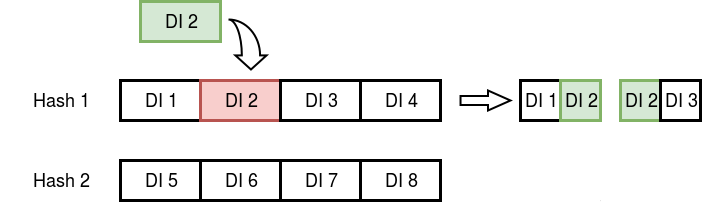
\includegraphics[width=1.0\textwidth]{pics/invalid.png}
	\caption{Перепроигрывание}
\end{figure}


\setmonofont[Mapping=tex-text]{CMU Typewriter Text}
\bibliographystyle{ugost2008ls}
\bibliography{diploma.bib}
\end{document}
